\subsection{Linear Transformations Between Abstract Vectors}

\begin{definition}[\textbf{Linear Transformation, Linear Map, Linearity}]
    \phantom{}\\
    If $V$ and $W$ are vector spaces over $\F$, a function $L:V\to W$ is called a \textbf{linear transformation}
    (or \textbf{linear map}) if it satisfies the \textbf{linearity} properties:
    \begin{enumerate}
        \item $L(\vx + \vy) = L(\vx) + L(\vy)$, and
        \item $L(c\vx) = cL(\vx)$
    \end{enumerate}
    \ $\forall \vx, \vy \in V$, $c \in \F$.
\end{definition}

\begin{remark}
    \phantom{}
    We can combine the two properties and check if $L(c\vx + \vy) = L(\vx) + L(\vy)$, $\forall \vx,\vy \in V$ and $c \in \F$.
\end{remark}

\begin{example}
    $\left[ \phantom{A} \right]:V\to \F^n$ is a linear map. 
\end{example}

\textbf{Question:} Does $L$ respect zero vector \& additive inverse?

\makebox[\linewidth]{\hrulefill}
{\large \textbf{Lecture 9}}

Well, I came late...

\begin{proposition}
    Let $L:V\to W$ be a linear map, and let $\vzero_V$ and $\vzero_W$ denote the zero vectors of $V$ and $W$, respectively.
    Then \[L(\vzero_V) = \vzero_W\]
\end{proposition}

\textbf{Observation}: The definition of "linear map" is essentially "a function that respects vector space structure".

Let $L:V\to W$ be a linear map. $L$ respects $+$ and $\cdot$. What else does it respect?
\begin{enumerate}[label=(\alph*)]
    \item Does a linear map respect $\vzero$? \\
    Yes! $L(\vzero_V) = L(0\cdot \vzero_V) = 0 \cdot L(\vzero_V) = \vzero_W$.
    \item Does a linear map respect additive inverse? \\
    Yes! $L(-\vx) = L((-1)\vx) = (-1)L(\vx) = -L(\vx)$.
    \item What else? Does L respect spans? Does L respect linear independence?
\end{enumerate}

\begin{example}[\textbf{Basic Examples \& Linear Maps}]
    \phantom{}
    \begin{enumerate}
        \item The zero map $L:V\to W$, $L(\vvv) = \vzero_W$, $\forall \vvv$ (Notation: can also write $\vvv \mapsto \vzero$).
        \item The identity map $L:V\to W$ or $\vvv \mapsto \vvv$, $L(\vvv) = \vvv$, $\forall \vvv$.
    \end{enumerate}
\end{example}

\begin{remark}
    Given a function $L:V \to W$, we will often write $\vvv \mapsto \vw$ to mean that $L$ sends $\vvv$ to $\vw$.
\end{remark}

\begin{example}[\textbf{Fundamental Examples}]
    \phantom{}
    \begin{enumerate}
        \item Let $\mB$ be an ordered basis for $V$. The coordinate map $[\phantom{A}]_{\mB} : V \to \F^n$ or $\vvv \mapsto \left[ \vvv \right]_{\mB}$ is a linear map. \\
        Special case: $V = \mP_3(\R)$, $\mB = \left\{ 1,x,x^2,x^3 \right\}$, then the $\mB$-coordinate map is
        $[\phantom{A}]_{\mB} : \mP_3(\R) \to \R^4$ $\left( a+bx+cx^2 + dx^3 \mapsto \left[ a+bx+cx^2 + dx^3 \right]_{\mB} = \cv{a \\ b \\ c \\d} \right)$.
        \item Let $A \in M_{m \times n}(\F)$. Define $L_A: \F^n \to \F^m$, $\vx \mapsto A\vx$ by $L_A(\vx) = A\vx$. This is linear. \\
        Special case: $A = \cv{1 & 1 & 1 \\ 2 & 3 & 4} \in M_{2 \times 3}(\F)$ and $L_A: \F^3 \to \F^2$, $\cv{a \\ b \\ c} \mapsto A\cv{a \\ b \\ c} = \cv{a+b+c \\ 2+3b+4c}$ .
    \end{enumerate}
\end{example}

\begin{example}[\textbf{More Examples}]
    \phantom{}
    \begin{enumerate}
        \item The differentiation map $D:\mP_n(\F) \to \mP_{n-1}(\F)$, $p(x)\mapsto p^\prime(x)$ is linear. $D(cp(x)+q(x)) = (cp(x)+q(x))^\prime = cp^\prime(x) + q^\prime(x) = cD(p(x)) + D(q(x))$. 
        \item The integration map $I: \mP_n(\F) \to \mP_{n+1}(\F)$ is linear. 
        \item The evaluation map, fix $\alpha \in \F$ in general is a linear map. Define $ev_\alpha : \mP_n(\F)\to \F$. \\
        Check: $\operatorname{ev}_\alpha(cp(x)+q(x)) = cp(\alpha) + q(\alpha) = c\operatorname{ev}_\alpha(p(x)) + \operatorname{ev}_\alpha(q(x))$.
        \item Transpose is linear. $L:M_{m \times n}(\F) \to M_{n \times m}(\F)$. \\
        Check:: $L(cA + B) = (cA+B)^T = (cA)^T + B^T = c(A^T) + B^T = cL(A) + L(B)$.
        \item Trace is linear. $\operatorname{tr}:M_{m \times n}(\F) \to \F$, $A \mapsto \operatorname{tr}(A)$.
    \end{enumerate}
\end{example}

\begin{example}[\textbf{Non-Linear Examples}]
    \phantom{}
    \begin{enumerate}
        \item Determinant is not linear except for $n$ = 1. $\operatorname{det}:M_{n \times n}(\F)\to \F$. \\
        If $n = 1$, this is linear (identity map $\F \to \F)$. \\
        If $n > 1$, $\det(A+B) \neq \det(A) + \det(B)$, and $\det(cA) = c^n\det(A) \neq c\det(A)$, in general. 
        \item $L:M_{2 \times 3}(\F) \to \mP_2(\F)$, $\cv{a & b & c \\ d & e & f} \mapsto (a+b) + (c+d)x + x^2$ is \underline{NOT} linear as it does not respect to $\vzero$, i.e. $L(\vzero) \neq \vzero$
        since $L\left( \cv{0 & 0 & 0 \\ 0 & 0 & 0} \right) = 0 + 0x + x^2 \neq 0 + 0x + 0x^2$. 
    \end{enumerate}
\end{example}

\textbf{Problem:} $L:\mP_2(\F) \to M_{2 \times 2}(\F)$ or $p(x) \mapsto \cv{p(1) & p^\prime(1) \\ p^\dprime(1) & p^\trprime(1)}$.
Is this linear? \\
Yes! (intuition: differentiation and evaluation are both liner) We will come back to this next lecture.


\subsection{Rank and Nullity}

* The two most important features of a linear map are:
\begin{enumerate}
    \item what it destroys
    \item what it creates.
\end{enumerate}
\vspace{-3mm}

\begin{figure}[htbp]
    \center
    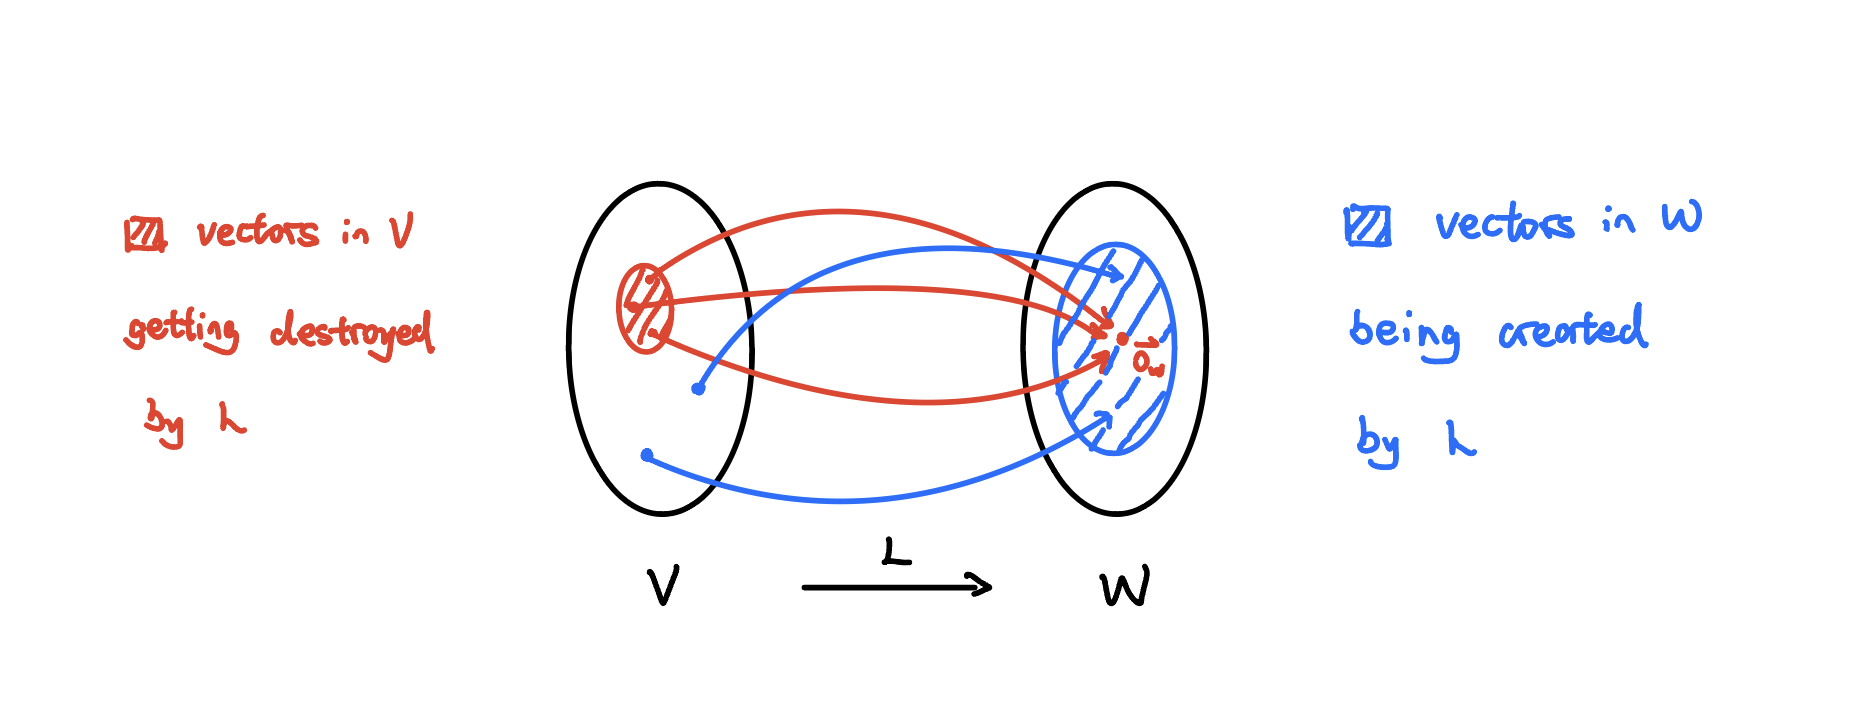
\includegraphics[scale=0.23]{img/linear-mapping.jpg}
    \caption{Two features of linear mapping.}
\end{figure}

\begin{definition}[\textbf{Kernel, Nullspace, Range}]
    \phantom{}\\
    Let $L:V\to W$ be a linear map. The \textbf{kernel} (or \textbf{nullspace}) of $L$ is
    \[\ker{(L)} = \left\{\vx \in V: L(\vx) = \vzero\right\}.\]
    The \textbf{range} (or \textbf{image}) of $L$ is
    \[\range{(L)} = \left\{  L(\vx) \in W: \vx \in V \right\}.\]
\end{definition}

\begin{remark}
    Kernel $\to$ vectors "destroyed" by $L$ \quad  \& \quad Range $\to$ vectors "created" by $L$. \\
    Referring to Figure 2 above, the red block represents $\ker(L)$, whereas the blue block represents $\range(L)$.
\end{remark}

\begin{note}
    $\ker(L) \subseteq V$ (domain) and $\range(L) \subseteq W$ (codomain).
\end{note}


\makebox[\linewidth]{\hrulefill}
{\large \textbf{Lecture 10}}

\begin{theorem}
    Let $V$ and $W$ be vector spaces over $\F$, and let $L:V\to W$ be a linear map. Then
    \begin{enumerate}[label={(\alph*)}]
        \item $\ker{(L)}$ is a subspace of $V$, and
        \item $\range{(L)}$ is a subspace of $W$.
    \end{enumerate}
\end{theorem}

\begin{proof}
    By the Subspace Test - Exercise.
\end{proof}

\begin{definition}[\textbf{Rank, Nullity}]
    Let $V$ and $W$ be vector spcaces over $\F$. The \textbf{rank} of a linear map $L:V\to W$ is the dimension of the range of $L$.
    The \textbf{nullity} of $L$ is the dimension of the kernel (nullspace) of $L$. That is,
    \[\rk{(L)} = \dim{(\range{(L)})} \quad \text{and} \quad \nully{(L)} = \dim{(\ker{(L)})}.\] 
\end{definition}

\begin{note}
    These are VERY important numerical invariants of $L$.
\end{note}

\begin{example}
    \phantom{}
    \begin{enumerate}
        \item Let $Z:V\to W$ be the zero map ($Z(\vvv) = \vzero \; \forall \vvv \in V$). Then $\ker(Z) = V$ and $\range(Z) = \{\vzero\}$.
        \item Idendity map $\text{id}:V \to V$ ($\operatorname{id}(\vvv) = \vvv$). Then $\ker(\text{id}) = \{\vzero\}$ and $\range(\text{id}) = V$.
        \item $\mB$-coordinates map. Suppose $\mB$ is an ordered basis for $V$ and $\dim(V) = n$, $[\phantom{A}]_{\mB}:V \to \F^n$ or $\vvv \mapsto [\vvv]_{\mB}$.
        Then, $\ker([\phantom{A}]_{\mB}) = \left\{ \vzero_V \right\}$. \vspace{-3mm}
        \begin{proof}
            Let $\vvv \in \ker([\phantom{A}]_{\mB}) \iff [\vvv]_{\mB} = \vzero_{\F^n} = \cv{0 \\ \vdots \\ 0} \iff \vvv = 0\vvb_1 + 0\vvb_2 + \cdots + 0\vvb_n$ 
            $\iff \vvv = \vzero_V$.
        \end{proof}

        And $\range([\phantom{A}]_{\mB}) = \F^n$. \vspace{-3mm}
        \begin{proof}
            $\range([\phantom{A}]_{\mB}) \subseteq \F^n$ by definition. So just need to prove $\supseteq$. Take $\cv{a_1 \\ a_2 \\ \vdots \\ a_n} \in \F^n$.
            Consider $\vvv = a_1\vvb_1 + a_2\vvb_2 + \cdots + a_n\vvb_n \in V$. Then $[\vvv]_{\mB} = \cv{a_1 \\ a_2 \\ \vdots \\ a_n}$, so $\cv{a_1 \\ a_2 \\ \vdots \\ a_n} \in \range([\phantom{A}]_{\mB})$.
        \end{proof}

        In addition, $\nully([\phantom{A}]_{\mB}) = 0$ and $\rk([\phantom{A}]_{\mB}) = \dim(\F^n) = n$.
        \item ***Matrix mapping. Let $A \in M_{m \times n}(\F)$. Let $L_A:\F^n \to \F^m$ or $\vx \mapsto A\vx$. Then $\ker(L_A) = \left\{ \vx \in \F^n: L_A(\vx) = \vzero \right\} = \left\{ \vx \in \F^n: A\vx = \vzero \right\} = \nul(A)$.
        
        And $\range(L_A) = \left\{ \vw \in \F^m: \vw = A\vx \text{ for some } \vx \in \F^n \right\} = \cdots = \col(A)$. (IMPORTANT: must be able to show this...)

        Also, $\nully(L_A) = \dim(\nul(A)) = \nully(A)$ and $\rk(L_A) = \dim(\col(A)) = \rk(A)$.
        \item Differentiation. $D:\mP_n(\F) \to \mP_{n-1}(\F)$ or $p(x) \mapsto p^\prime(x)$.\\
        Then $\ker(D) = \left\{ a_01+0x+0x^2+\cdots +0x^n: a_0 \in \F \right\} = \spn{\{1\}}$.
        \begin{proof}
            \begin{align*}
                p(x) = a_0+a_1x+\cdots +a_nx^n \in \ker(D) &\iff p^\prime(x) = \vzero \\
                &\iff a_12a_2x+\cdots +na_nx^n = 0+0x+\cdots +0x^n \\
                &\iff a_1 = a_2 = \cdots = a_n = 0 \\
                &\iff p(x) = a_11
            \end{align*}
        \end{proof}

        And $\range(D) = \mP_{n-1}(\F)$. 
        \begin{proof}
            Given $a_0+a_1x+a_2x^2 + \cdots +a_{n-1}x^{n-1} = D(a_0x + \frac{1}{2}a_1x^2 + \cdots + \frac{a_{n-1}}{n}x^n)$.
            So every $p(x) \in \mP_{n-1}(\F)$ is $D(\text{something})$ and is in $\range(D)$.

            Also, $\nully(D) = \dim(\ker(D)) = \dim(\spn{\{1\}}) = 1$ and $\rk(D) = \dim(\range(D)) = \dim(\mP_{n-1}(\F)) = n$.
        \end{proof}
    \end{enumerate}
\end{example}


\makebox[\linewidth]{\hrulefill}
{\large \textbf{Lecture 11}}

Warm-up: Let $L:\R^3 \to \mP_1(\R)$ be defined by $L\left( \cv{a \\ b \\ c} \right) = (a+b+c)x$. Find $\rk(L)$ and $\nully(L)$.  \\
\textbf{Solution:} Since $\rk(L) = \dim(\range(L))$, we can claim the following by inspection (intuition). 

\textbf{Claim:} $\range(L) = \spn\{x\}$.
\begin{proof}
    For ($\Rightarrow$), \vspace{-8mm}
    \begin{align*}
        p(x) \in \range(L) &\iff p(x) = L\left( \cv{a \\ b \\ c} \right) \text{ for some $\cv{a \\ b \\ c} \in \R^3$}. \\
        &\iff p(x) = (a+b+c)x \\
        &\iff p(x) \in \spn\{x\}.
    \end{align*}
    
    \vspace*{-5mm}For ($\Leftarrow$), take $\alpha x \in \spn\{x\}$ and note that $\alpha x = L \left( \cv{\alpha \\ 0 \\ 0} \right)$, so $\alpha x \in \range(L)$.

    Therefore, we have $\rk(L) = \dim(\range(L)) = \dim(\spn\{x\}) = 1$.
\end{proof}

Next, for $\nully(L)$, we know that $\nully(L) = \dim(\ker(L))$. Then \vspace{-4mm}
\begin{align*}
    \cv{a \\ b \\ c} \in \ker(L) &\iff L \left( \cv{a \\ b \\ c} \right) = 0 + 0x \\
    &\iff (a+b+c)x = 0 + 0x \\
    &\iff a+b+c = 0 \\
    &\iff a = -b-c \\
    &\iff \cv{a \\ b \\ c} = \cv{-b-c \\ b \\ c} = b\cv{-1 \\ 1 \\ 0} + c\cv{-1 \\ 0 \\ 1}.
\end{align*}

Therefore, $\ker(L) = \spn \left\{ \cv{-1 \\ 1 \\ 0}, \cv{-1 \\ 0 \\ 1} \right\}$ and the two vectors are clearly linearly independent. Thus, $\nully(L) = \dim(\ker(L)) = 2$.

\begin{remark}
    This warm-up example leads to the following important theorem.
\end{remark}

\begin{theorem}[\textbf{Rank-Nullity Theorem}]
    \phantom{}\\
    Let $V$ and $W$ be vector spaces over $\F$ with $V$ finite-dimensional and $\dim{(V)} = n$.
    Let \\ $L:V\to W$ be a linear map. Then $\rk{(L)}+\nully{(L)} = n$.
\end{theorem}

\begin{remark}
    This is also refered to the Fundamental Theorem of Linear Algebra.
\end{remark}

\textbf{Important Fact} from Linear Algebra 1: $\dim(\null(A)) = \nully(A)$ and $\dim(\col(A)) = \rk(A)$.

\begin{example}
    \phantom{}
    \begin{enumerate}
        \item Consider the $\mB$-coordinate map $[\phantom{A}]_{\mB}:V \to \F^n$, where $V$ is n-dimensional.
        By definition, $\range([\phantom{A}]_{\mB}) = \F^n$, so $\rk([\phantom{A}]_{\mB}) = n \implies \nully([\phantom{A}]_{\mB}) = 0$.
        \item Consider $\operatorname{tr}:M_{n \times n}(\F) \to \F$. Let $W = \ker(\operatorname{tr}) = \left\{ A \in M_{n \times n}(\F): \operatorname{tr}(A) = 0 \right\}$.
        What is $\dim(W)$? \\
        \textbf{Solution:} $\dim(W) = nully(\operatorname{tr}) = \dim(M_{n \times n}(\F)) - \rk(\operatorname{tr}) = n^2 - 1$. \\
        Note that $\rk(\operatorname{tr}) = 1$ because $\rk(\operatorname{tr}) = \dim(\range(\operatorname{tr}))$ and $\range(\operatorname{tr})$ is a subspace of $\F$.
        But $\F$ only has two subspaces, $\{\vzero\}$ and itself. So $\range(\operatorname{tr}) = \F$.
        \item (Exercise): $L:V \to \F$ is a non-zero map. Prove that $\nully(L) = \dim(V) - 1$.
    \end{enumerate}
\end{example}

\begin{definition}[\textbf{Injective, Surjective}]
    \phantom{}\\
    The linear map $L:V \to W$ is
    \begin{enumerate}[label=(\alph*)]
        \item \textbf{injective} (or \textbf{one-to-one}) if $\ker(L) = \{\vzero\}$ ($\iff \nully(L) = 0$ )
        \item \textbf{surjective} (or \textbf{onto}) if $\range(L) = W$ ($\iff \rk(L) = \dim(W)$ ).
    \end{enumerate}
\end{definition}

\begin{example}
    $\tra:M_{n \times n}(\F) \to \F$. \\
    $\tra$ is surjective since $\rk(\tra) = 1 = \dim(\F)$. But $\tra$ is not injective since $\nully(\tra) = n^2 - 1 \neq 0$ when $n \neq 1$.
\end{example}

\pagebreak
 
\makebox[\linewidth]{\hrulefill}
{\large \textbf{Lecture 12}}

\begin{example}
    \phantom{}
    \item $L:M_{2 \times 2}(\R) \to \mP_2(\R)$, $\cv{a & b \\ c & d} \mapsto a + (b+c)x + (a-2d)x^2$. Is $L$ injective? Surjective?
        
        \textbf{Solution 1:} (Direct from definition) \\
        For $\ker(L)$: \vspace{-4mm}
        \begin{align*}
            \cv{a & b \\ c & d} \in \ker(L) &\iff a + (b+c)x + (a-2d)x^2 = \vzero \\
            &\iff a=0, b+c=0, a-2d=0 \\
            &\phantom{if}\vdots \\
            &\iff a=d=0, c=-b \\
            &\iff \cv{a & b \\ c & d} = \cv{0 & b \\ -b & 0} = b\cv{0 & 1 \\ -1 & 0}
        \end{align*}
        \vspace{-2mm}Therefore, $\ker(L) = \spn \left\{ \cv{0 & 1 \\ -1 & 0} \right\}$. Thus $L$ is not injective since $\ker(L) = \{\vzero\}$. \\

        For $\range(L)$: \vspace{-4mm}
        \begin{align*}
            p(x) \in \range(L) &\iff p(x) = a + (b+c)x + (a-2d)x^2 \\
            &\iff p(x) = a(1+x^2) + bx + cx + d(-2x^2) \\
            &\iff p(x) \in \spn\{1+x^2, x, x, -2x^2\}
        \end{align*}
        Therefore $\{1+x^2, x, -2x^2\}$ is linearly independent and hence a basis for $\range(L)$. So $\rk(L) = \dim(\range(L)) = 3 = \dim(\mP_2(\R))$, $L$ is surjective.

        \vspace{2mm}
        \textbf{Solution 2:} (Try Rank-Nullity Theorem) \\
        We have, $\dim(M_{2 \times 2}(\R)) = 4 = \rk(L) + \nully(L)$. Once we have rank \textbf{OR} nullity, we get the other one! This cuts work in half. \\
        Since $\dim(\mP_2(\R)) = 3$, then $\rk(L) \leq \dim(\mP_2(\R)) = 3 \implies \nully(L) \neq 1$. Thus, $L$ is not injective.

        \begin{note}
            Don't forget that we still need to show some work to check surjective if using solution 2.
        \end{note}
\end{example}

\begin{theorem}
    \phantom{}
    Let $L:V \to W$ be a linear map between finite-dimensional vector spaces. 
    \begin{enumerate}[label=(\alph*)]
        \item If $\dim(V) > \dim(W)$, then $L$ cannot be injective.
        \item If $\dim(V) < \dim(W)$, then $L$ cannot be surjective. 
        \item If $\dim(V) = \dim(W)$, then $L$ is injective $\iff$ if $L$ is surjective.
    \end{enumerate}
\end{theorem}

\begin{proof}
    We will prove (a).
    
    By Rank-Nullity Theorem, we have $\dim(V) = \nully(L) + \rk(L)$. And $\rk(L) = \dim(\range(L)) \leq \dim(W) < \dim(V)$. If $\nully(L) = 0$,
    then $\dim(V) = \rk(L) < \dim(V)$, a contradiction!
\end{proof}

\begin{example}[Above Example Continued]
    \phantom{}\\
    $L:M_{2 \times 2}(\R) \to \mP_2(\R)$, $\cv{a & b \\ c & d} \mapsto a + (b+c)x + (a-2d)x^2$. \\
    This looks a lot like $T: \R^4 \to \R^3$, $\cv{a \\ b \\ c \\ d} \mapsto \cv{a \\ b+c \\ a-2d}$.
\end{example}

\begin{remark}[\textbf{Refresher}]
    Every linear map $T: \R^n \to \R^m$ is given by a matrix $T(\vx) = A\vx$ for some $A \in M_{m \times n}(\R)$.
    For our example: $T: \R^4 \to \R^3$, $\cv{a \\ b \\ c \\ d} \mapsto \cv{a \\ b+c \\ a-2d}$. We want $A \in M_{3 \times 4}(\R)$ so that
    $T\left( \cv{a \\ b \\ c \\ d} \right) = A\cv{a \\ b \\ c \\ d} = \cv{a \\ b+c \\ a-2d}$. We discover: $A =
    \begin{bmatrix}
        1 & 0 & 0 & 0 \\
        0 & 1 & 1 & 0 \\
        1 & 0 & 0 & -2
    \end{bmatrix}.$ \\

    \vspace{-2mm}\textbf{Summary:} If $T: \R^n \to \R^m$, let $A = 
    \begin{bmatrix}
        | & | & | \\
        T(\ve_1) & \cdots & T(\ve_n) \\
        | & | & |
    \end{bmatrix}$,
    then $T(\vx) = A\vx$.
    \begin{note}
        $A$ knows everything about $T$!!!
    \end{note}
\end{remark}


\makebox[\linewidth]{\hrulefill}
{\large \textbf{Lecture 13}}


% \subsection{Linear Maps as Matrices}

% \begin{theorem}
%     Let $V$ be an $n$-dimensional vector space with ordered basis $\mB$. Let $W$ be an $m$-dimensional vector space
%     with ordered basis $\mC$. Then, for every linear map $L:V\to W$, $\exists$ an $m \times m$ matrix $A$ \st
%     $[L(\vvv)]_{\mC} = A[\vvv]_{\mB}$ $\forall \vvv \in V$. Conversely, every $m \times m$ matrix $A$ defines a linear map $L:V\to W$
%     by $[L(\vvv)]_{\mC} = A[\vvv]_{\mB}$.
% \end{theorem}

% \begin{corollary}
%     Let $V$ be a vector space with ordered basis $\mB = \left\{  \vvb_1,\ldots,\vvb_n \right\}$. let $W$ be a vector space with ordered basis
%     $\mC = \left\{  \vc_1,\ldots,\vc_m \right\}$. Let $L:V\to W$ be a linear map. Then the $m \times n$ matrix $A$ \st $[L(\vvv)]_{\mC} = A[\vvv]_{\mB}$
%     $\forall \vvv \in V$, which we denote $\prescript{}{\mC}{\left[  L \right]_{\mB}}$, is given by
%     \[\prescript{}{\mC}{\left[  L \right]_{\mB}} = \left[  [L(\vvb_1)]_{\mC} \cdots [L(\vvb_n)]_{\mC} \right].\]
% \end{corollary}

% \begin{definition}[\textbf{Matrix of a Linear Map}]
%     \phantom{}\\
%     We call the matrix $\prescript{}{\mC}{\left[  L \right]_{\mB}}$ the \textbf{matrix of the linear map} $L:V\to W$ with respect to the ordered bases $\mB$ and $\mC$ pf $V$ and $W$, respectively. \\
%     \phantom{}\\
%     If $V = W$, so that $L:V\to V$, and we choose the same basis $\mB$ for both the domain and codomain of $L$, then we will write $[L]_{\mB}$ insted of $\prescript{}{\mB}{[L]_{\mB}}$.
% \end{definition}

% \begin{proposition}
%     Let $V$, $U$, and $W$ be vector spaces over $\F$ with bases $\mB$, $\mC$, and $\mD$ respectively. Let $L:V\to U$
%     and $M:U\to W$ be linear maps. Then $\prescript{}{\mD}{\left[  M \circ L \right]_{\mB}} = \prescript{}{\mC}{\left[  M \right]_{\mC}} \prescript{}{\mC}{\left[  L \right]_{\mB}}$.
% \end{proposition}

% \begin{definition}[\textbf{Column Space, Rank, Nullspace, Nullity of a Matrix}]
%     \phantom{}\\
%     Let $A \in M_{m \times n}(\F)$. \\
%     \phantom{}\\
%     The \textbf{column space} of $A$, denoted by $\col{(A)}$, is the span of the columns of $A$.
%     The \textbf{rank} of $A$ is the dimension of its column space:
%     \[\rk{(A)} = \dim{(\col{(A)})}. \\\]
%     The \textbf{nullspace} of $A$, denoted by $\null{(A)}$, is the set of $\vvv \in \F^n \st A\vvv = \vzero$.
%     The \textbf{nullity} of $A$ is the dimension of its nullspace:
%     \[\nully{(A)} = \dim{(\null{(A)})}.\] 
% \end{definition}

% \begin{proposition}
%     Let $L:V\to W$ be a linear map between finite-dimensional vector spaces, and let $A = \prescript{}{\mC}{\left[  L \right]_{\mB}}$,
%     where $\mB$ and $\mC$ are ordered bases for $V$ and $W$ respectively.
%     \begin{enumerate}[label={(\alph*)}]
%         \item $\vvv \in \ker{(L)} \iff \left[  \vvv \right]_{\mB}$.
%         \item $\vw \in \range{(L)} \iff \left[  \vw \right]_{\mC}$.
%     \end{enumerate}
% \end{proposition}



% \subsection{Change of Coordinates}

% \begin{definition}[\textbf{Change of Coordinates Matrix}]
%     Let $V$ be a finite dimensional vector space, and let $\mB$ and $\mC$ be two bases for $V$.
%     The \textbf{change of coordinates matrix} $\prescript{}{\mC}{I_{\mB}}$ is the matrix $\prescript{}{\mC}{\left[  \text{id} \right]_{\mB}}$,
%     where $\text{id}:V\to V$ is the identity map.
% \end{definition}

% \begin{proposition}
%     Let $V$ be a finite dimensional vector space with bases $\mB$ and $\mC$. Then $\prescript{}{\mC}{I_{\mB}} = \left(  \prescript{}{\mB}{I_{\mC}} \right)^{-1}$.
% \end{proposition}


% \subsection{Isomorphisms of Vector Spaces}

% \begin{definition}[\textbf{Injective (One-to-One), Surjective (Onto)}]
%     \phantom{}\\
%     Let $L:V\to W$ be a linear map between vector spaces and let $\vvv_1$, $\vvv_2 \in V$. \\
%     \phantom{}\\
%     We say $L$ is \textbf{injective} (or \textbf{one-to-one}) if $L(\vvv_1) = L(\vvv_2) \implies \vvv_1 = \vvv_2$. \\
%     We say $L$ is \textbf{surjective} (or \textbf{onto}) if $\range{(L)} = W$.
% \end{definition}

% \begin{lemma}
%     A linear map $L:V\to W$ is injective $\iff \ker{(L)} = \left\{ \vzero \right\}$.
% \end{lemma}

% \begin{proposition}
%     \phantom{}\\
%     Let $L:V\to W$ be a linear map between finite-dimensional vector spaces. Then
%     \begin{enumerate}[label={(\alph*)}]
%         \item $L$ is injective $\iff \nully{(L)} = 0$.
%         \item $L$ is surjective $\iff \rk{(A)} = \dim{(W)}$.
%     \end{enumerate}
    
% \end{proposition}

% \begin{definition}[\textbf{Isomorphism, Isomorphic}]
%     \phantom{}  \\
%     Let $L:V\to W$ be a linear map. If $L$ is both injective and surjective, we say $L$
%     is an \textbf{isommorphism}.    \\
%     If there is an isomorphism $L: V \to W$, we say that $V$ and are \textbf{isomorphic} to $W$,
%     and write $V \cong W$.
% \end{definition}

% \begin{proposition}
%     Let $L:V\to W$ be a linear map between finite-dimensional vector spaces, and let $A = \prescript{}{\mC}{\left[ L \right]_{\mB}}$,
%     where $\mB$ and $\mC$ are ordered bases for $V$ and $W$ respectively.
%     \begin{enumerate}[label={(\alph*)}]
%         \item $\ker{(L)} \cong \null{(A)}$.
%         \item $\range{(L)} \cong \col{(A)}$.
%     \end{enumerate}
% \end{proposition}

% \begin{proposition}
%     Let $V$ be an $n$-dimensional vector space over $\F$. If $\mB$ is an ordered basis for $V$, then the coordinate map
%     $\left[ \phantom{A} \right]_{\mB}:V\to \F^n$ defined by sending $\vvv$ to $\left[ \vvv \right]_{\mB}$ is an isomorphism.
% \end{proposition}

% \begin{proposition}
    
% \end{proposition}

% \begin{proposition}
    
% \end{proposition}

% \begin{theorem}
%     Suppose $V$ and $W$ are finite-dimensional vector spaces over the same field $\F$. Then $V \cong W \iff \dim{(V)} = \dim{(W)}$.
% \end{theorem}

% \begin{corollary}
%     Let $V$ be an $n$-dimensional vector space over $\F$. Then $V \cong F^n$.
% \end{corollary}

% \begin{proposition}
    
% \end{proposition}

% \begin{corollary}[\textbf{Range-Nullity Theorem for Matrices}]
    
% \end{corollary}

% \begin{proposition}
    
% \end{proposition}

% \begin{proposition}
    
% \end{proposition}

% \begin{proposition}
    
% \end{proposition}







\newpage